\section{Bubble sort}
\subsection{Aim}
To perform bubble sort on a list of numbers

\subsection{Code}
\begin{lstlisting}
DATA SEGMENT
  arr DW 1000H, 3000H, 4000H, 2000H
  count DW 4
DATA ENDS

CODE SEGMENT
ASSUME CS:CODE, DS:DATA
START:
  MOV AX, DATA
  MOV DS, AX
  XOR CX, CX
  XOR BX, BX

LOOP1:
  CMP CX, count
  JE EXIT
  XOR BX, BX
  LEA SI, arr
LOOP2:
  MOV AX, count
  SUB AX, CX
  SUB AX, 1
  CMP BX, AX
  JGE INCRLOOP1
  MOV AX, [SI]
  CMP AX, [SI+2]
  JL INCRLOOP2
  MOV AX, [SI]
  MOV DX, [SI+2]
  MOV [SI], DX
  MOV [SI+2], AX
INCRLOOP2:
  INC BX
  ADD SI, 2
  JMP LOOP2
INCRLOOP1:
  INC CX
  JMP LOOP1

EXIT:
  MOV AX, 4CH
  INT 21H
CODE ENDS
END START
\end{lstlisting}

\subsection{Output}
\begin{center}
	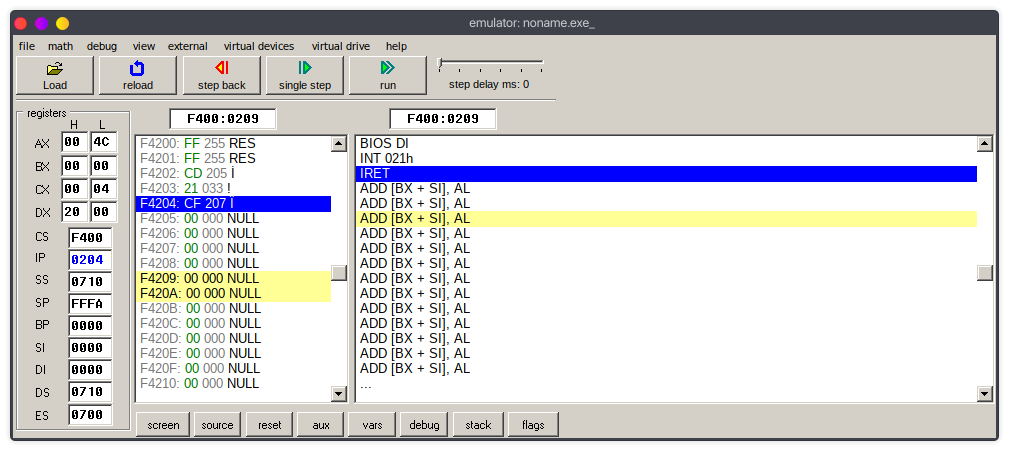
\includegraphics[width=0.90\textwidth]{img/p9/ss1.png}
	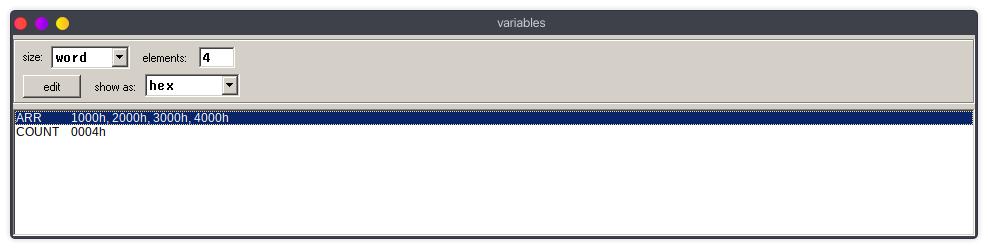
\includegraphics[width=0.90\textwidth]{img/p9/ss2.png}
\end{center}

\subsection{Result}
A 32bit array was sorted using bubble sort algorithm in emu8086